\chapter{Articles and their categories\label{cha:articles}}

This chapter analyses the core categories present in selected articles within the contextual background of the matches. Of the 122 corpus texts, 23 articles were analysed for this closer examination into how cultural diplomacy was represented in the match reports published by \textit{Neues Deutschland}. The articles cover the range of matches dating from the GDRNT's first World Cup Qualifying match against Finland in October 1972 through to the GDR’s World Cup Finals match against Chile in June 1974. The articles reported on different types of matches, ranging from friendly matches where teams would play each other with no competitive ramifications to World Cup Qualification matches and World Cup Finals matches. The match reports were typically published the day after the game, with some away matches having reported a few days later. Whilst most of the match reports were written by Max Schlosser, some were co-written by Horst Richter, Werner Klein, Wolfgang Richter, Eckhardt Galley and Klaus Ullrich\footnote{Chapter 4 provides more detail on Klaus Ullrich who held the position of Head of Sports at \textit{Neues Deutschland}.}. Five match reports had no credited author. Figure 3.1 lists the GDRNT’s matches with their corresponding \textit{Neues Deutschland} match report.

Figure 3.2 provides some contextual information around the matches the GDRNT played. The GDRNT were quite successful in the time period of the selected articles claiming 18 victories, 3 draws and 2 losses. Of the 23 matches, 15 were friendly matches, 6 were World Cup Qualifying (WCQ) matches and 2 were World Cup Finals (WCF) matches. The total amount of codes related to the core categories are listed within the column of the category itself. The codes capture instances in the data where the \textit{Neues Deutschland} journalists employ processes of ascription or evaluation related to the core categories.

The opponent’s Cold War alliance is also listed. For the purposes of this study, only countries who were signatory members to the North Atlantic Treaty Organisation (NATO) or the Warsaw Treaty Organization (Warsaw Pact) during 1972-1974 were classified as being part of that alliance. Both NATO and Warsaw Pact were military alliances that were in opposition to each other during the Cold War. The GDR itself was a member of the Warsaw Pact alliance (\cite{wagner2012}). Of the GDRNT opponents, Belgium, England, Iceland and Norway were members of NATO whereas Hungary, Romania and the Soviet Union were Warsaw Pact members (\cite{wagner2012}). Albania was an original member of the Warsaw Pact but left the alliance during the Soviet-Albanian split of 1961 in protest after the Warsaw Pact members had invaded Czechoslovakia (\cite{lüthi2007}, p. 480). Algeria was originally included within NATO’s strategic theatre as a colony of France (\cite{thomas2000}, p. 158) but terminated its affiliation with the alliance after it gained its independence from France following the aftermath of the Algerian War (\cite{connelly2002}).

\newpage
\begin{figure}[t]
\caption{GDRNT football matches and their match reports}
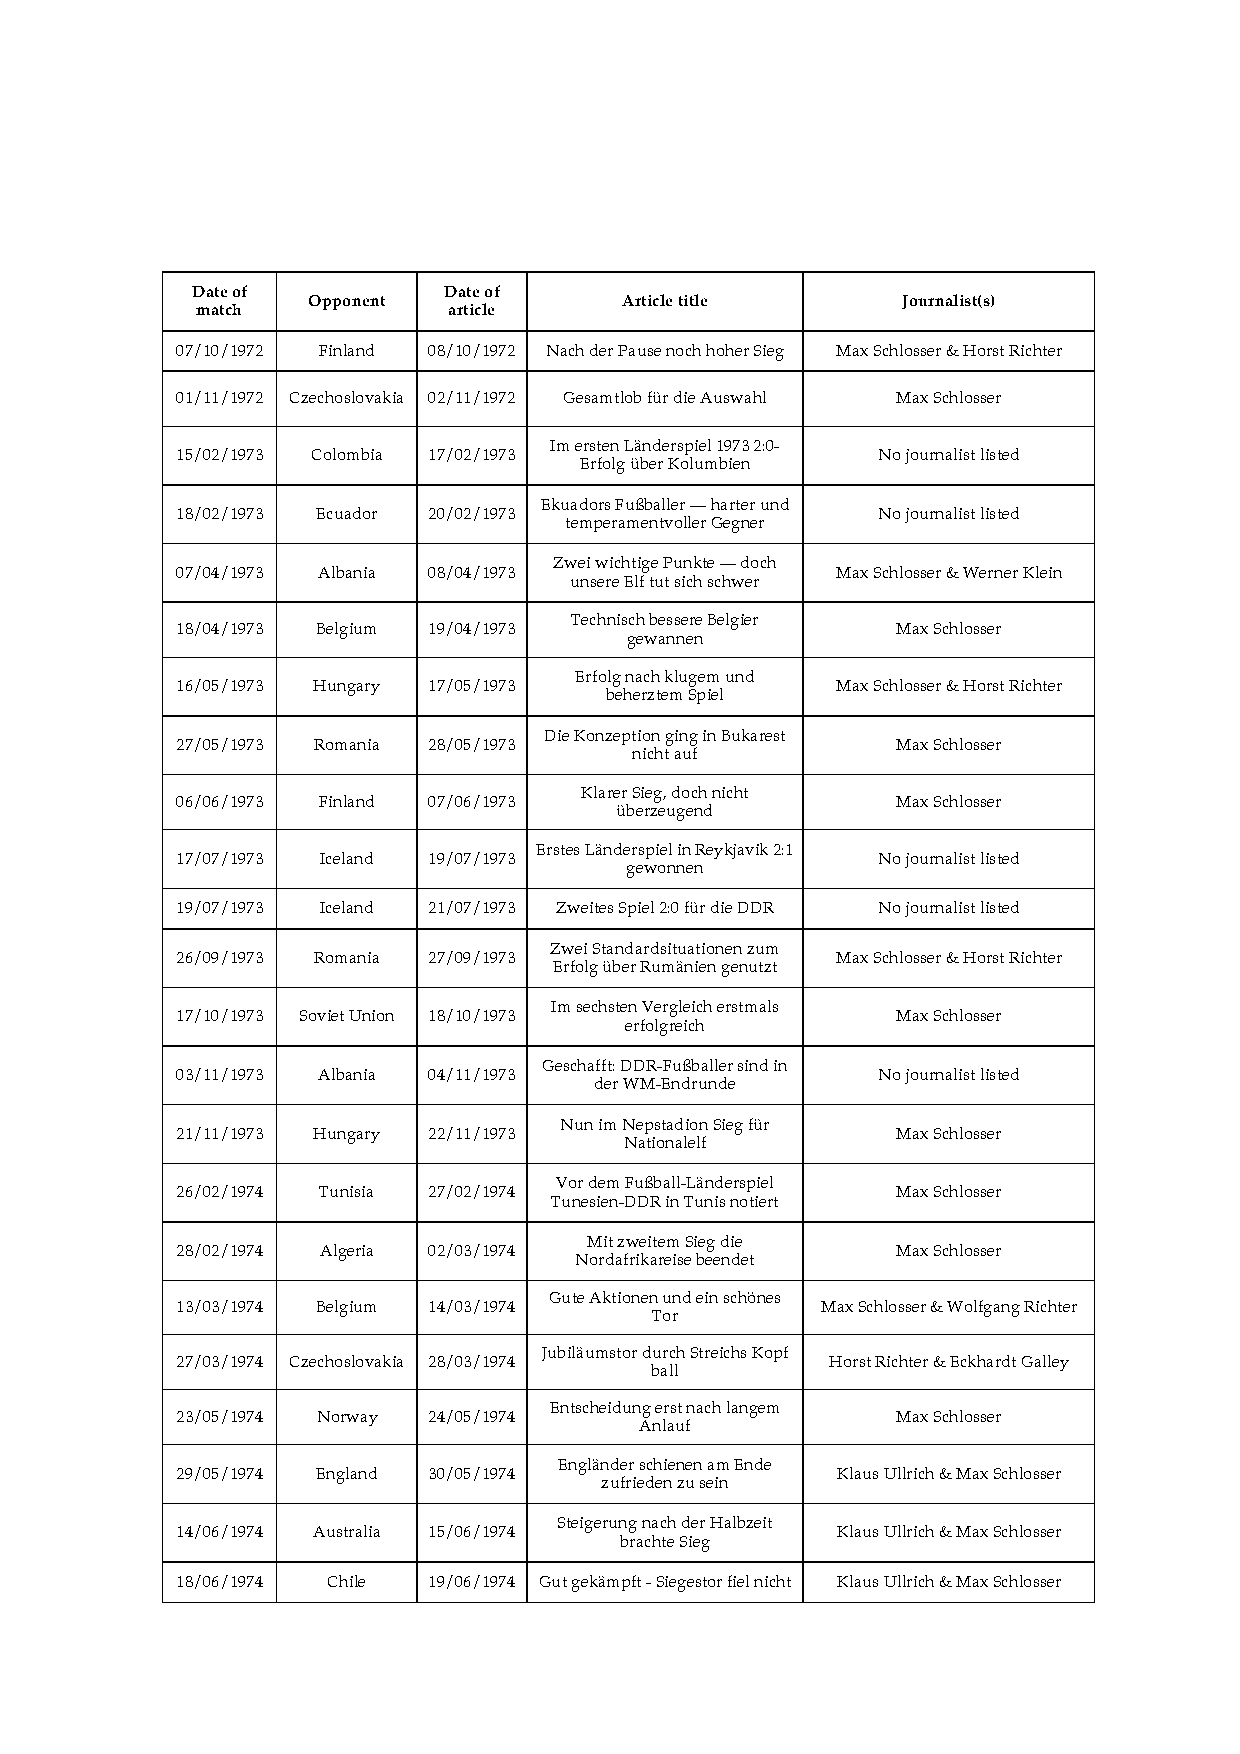
\includegraphics[width=\textwidth]{mres/images/figure 3.1.pdf}
\centering
\label{fig:fig3.1}
\end{figure}

\newpage
\begin{landscape}
\begin{figure}[!h]
\centering
\caption{Game context and number of coded references in categories}
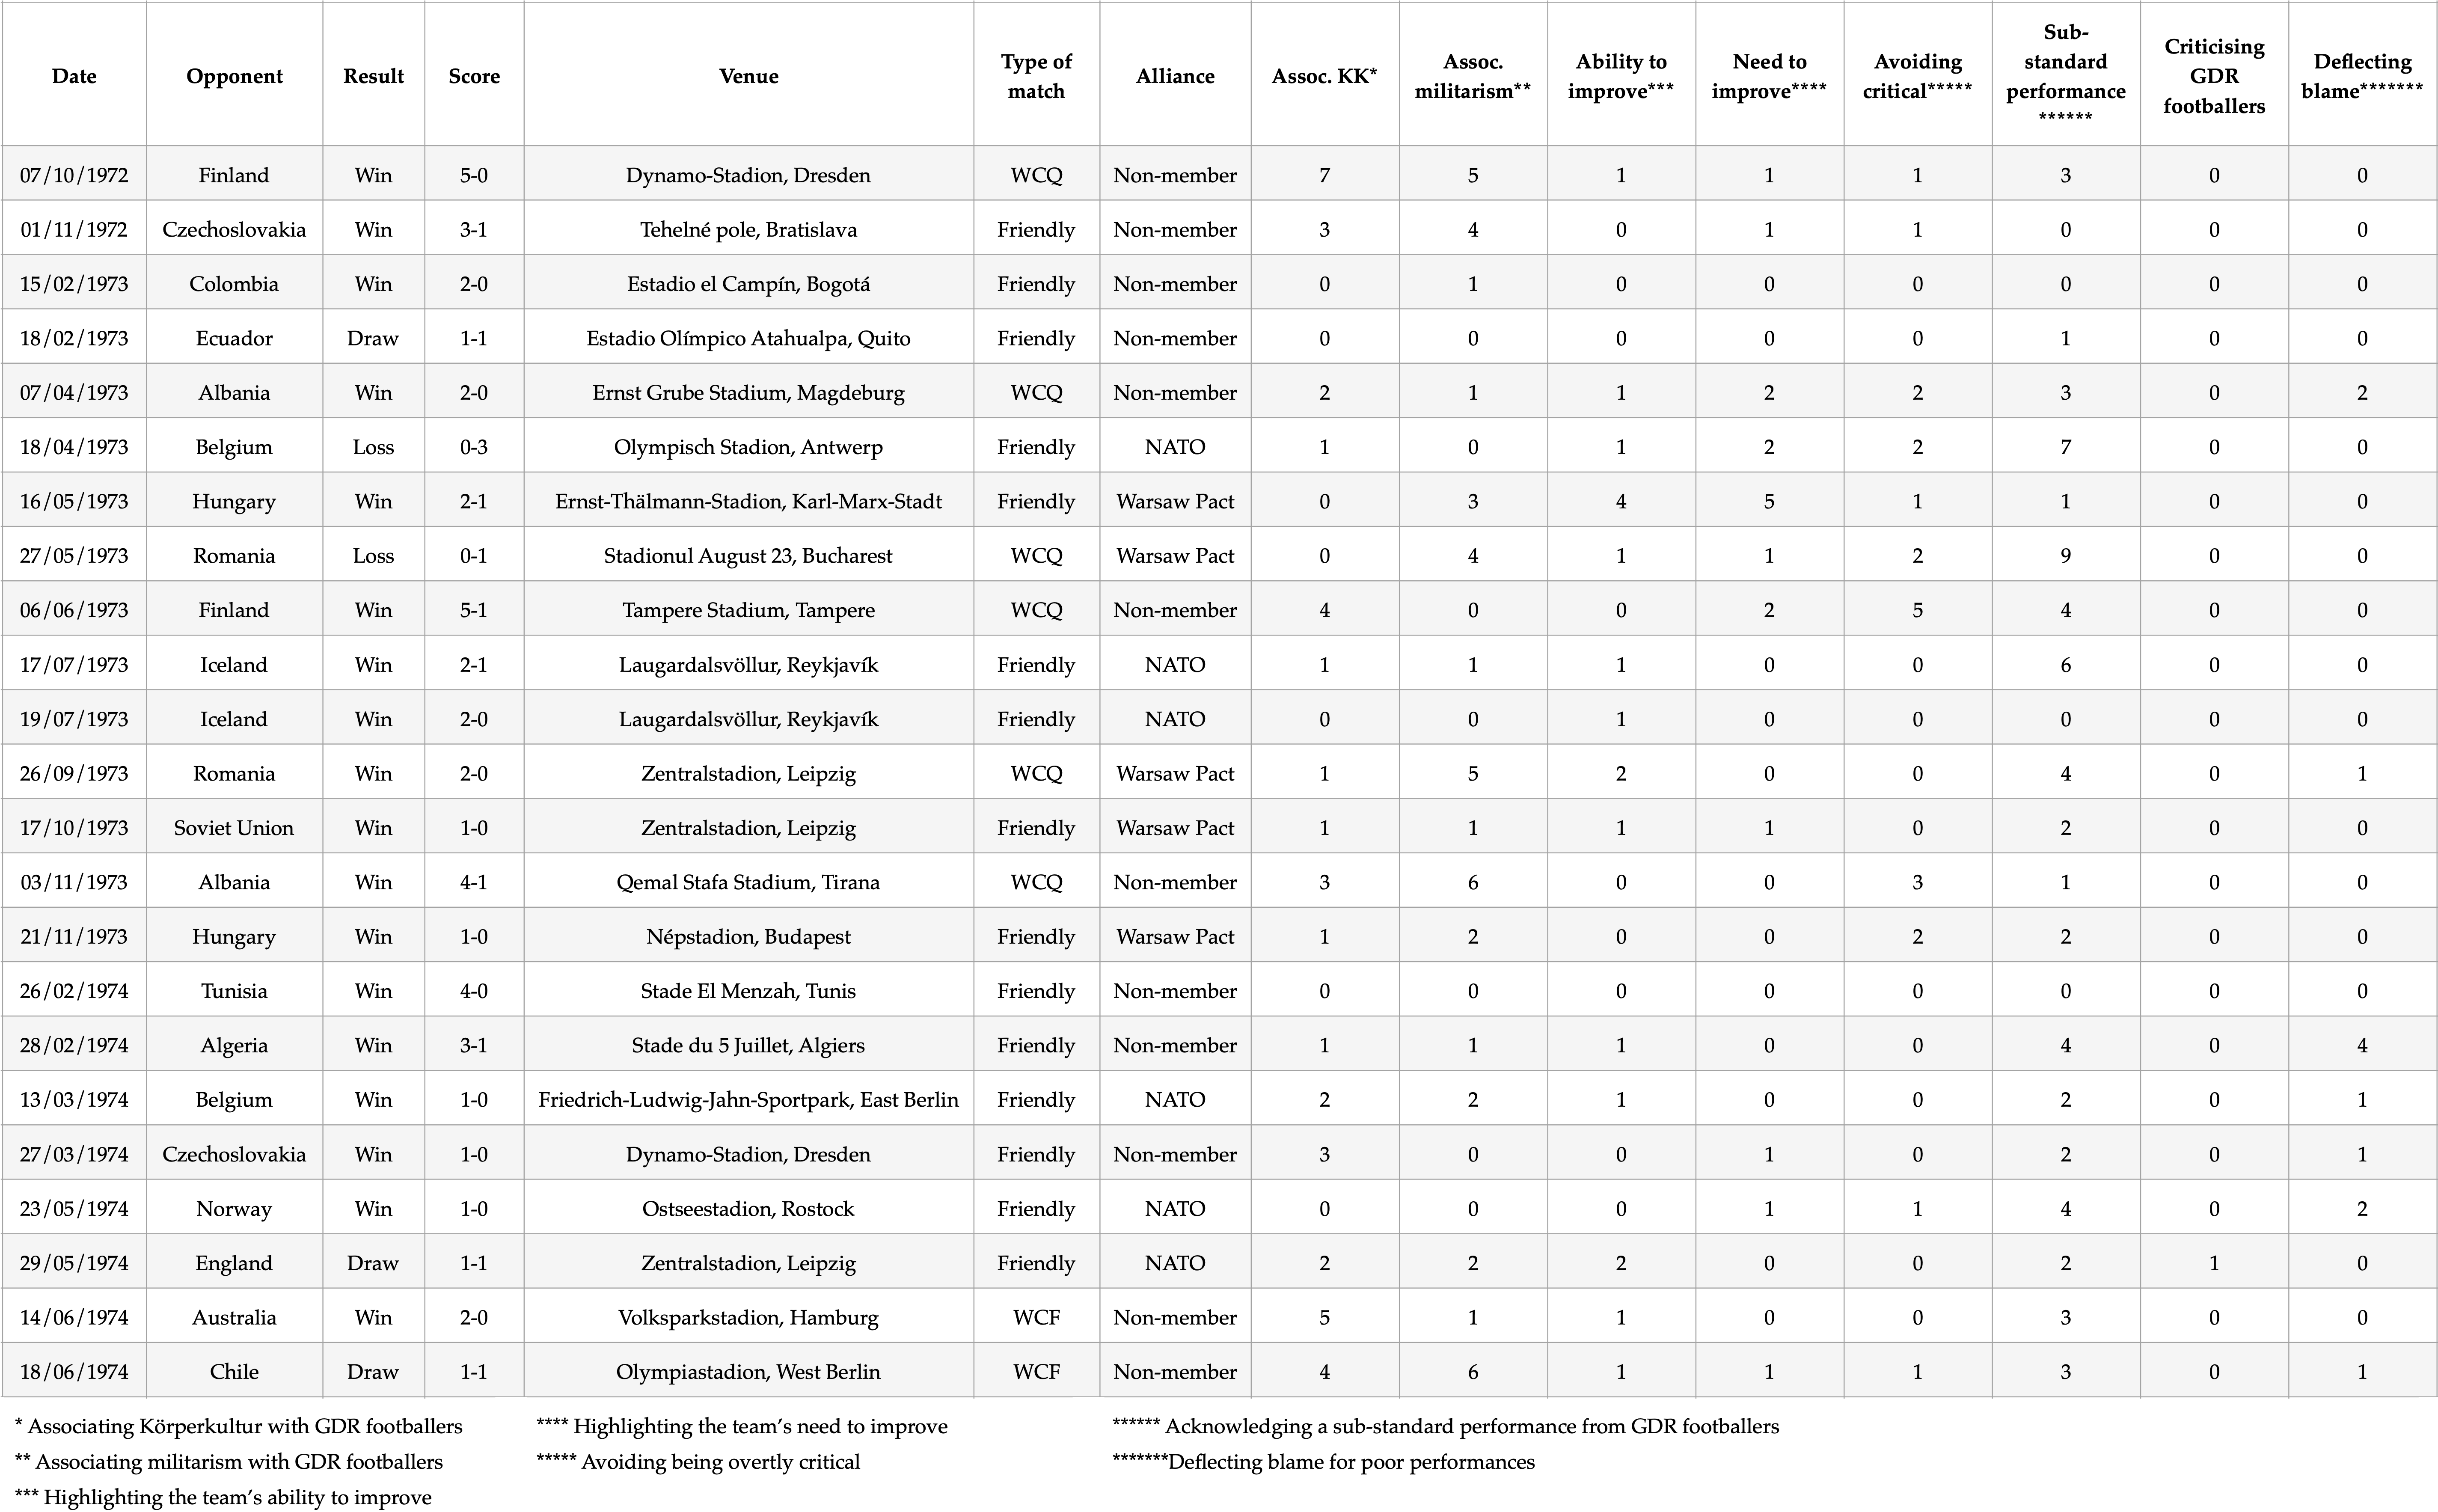
\includegraphics[width=\linewidth]{mres/images/figure 3.2.png}
\end{figure}
\end{landscape}

\section*{Article analyses}

The following section examines articles for the core categories to identify trends in the data. To achieve a deeper understanding of how categories work within and across articles, I analyse the match reports that cover the GDRNT’s largest victory and heaviest loss along with a wider examination across groups of articles that pertain to certain classifications. These classifications include the type of football match (friendly, WCQ and WCF) or whether the opponent was a member of NATO, Warsaw Pact or had no alliance membership. 

\subsection*{Single article analyses}

\subsubsection*{Largest victory}

\textbf{\textit{German Democratic Republic 5 – 0 Finland
\newline World Cup Qualifier, Dresden, 7th of October 1972.}}

The match report published on the 8th of October 1972 titled \textit{Nach der Pause noch hoher Sieg} (Big win after the break) covers the GDR’s first game in their World Cup Qualification campaign against Finland. The match was played in the Dynamo-Stadion in the city of Dresden. The 5-0 success was the GDR’s largest victory in the nation’s World Cup history (\cite{dähn2013}).

The most emphatic win for the GDR in the time of the articles analysed coincides with the highest amount of references to the category \textit{Associating Körperkultur with GDR footbal}l from all the articles analysed. The first coded reference to the category appears in the subtitle of the article, where journalists Max Schlosser and Horst Richter claim that the GDRNT’s physical conditioning was central to their victory: ‘Gäste konnten nach einer Stunde konditionell nicht mehr mithalten’ (Guests couldn't keep up with their [GDRNT] fitness levels after an hour) (\cite{nd19721008}). The main body of the article also references a change in the match’s tempo brought about by the speed of the GDRNT’s play: ‘Die endgültige Entscheidung bahnte sich nach rund einer Stunde an, als die DDR-Mannschaft das Tempo verschärfte und die Gäste kräftemäßig abbauten.’ (The final decision was made after about an hour, when the GDR team stepped up the pace and reduced the strength of the guests.’ (\cite{nd19721008}). The majority of the category’s references came from the summary of goals at the end of the article. \textit{Schnell} (quick) was the most commonly used adjective when describing either the GDRNT’s performance or the players themselves. The summary of goals also makes mention of other football actions such as ‘millimetergenauem Zuspiel’ (millimetre-precise delivery) and ‘langen Dribbling’ (long dribbling) (\cite{nd19721008}), emphasising the technical ability of GDR footballers.

\textit{Nach der Pause noch hoher Sieg} contained the second-highest amount of references to the category \textit{Associating militarism with GDR football} from all the articles analysed. The conceptual metaphor that imagines football as a battle was evident from the coded references. Stem variations of the word \textit{Kampf} were present within the article where Schlosser and Richter described when GDRNT players were engaged in ‘Zweikämpfen mit den robusten Gegenspielern’ (Duels with robust opponents) (\cite{nd19721008}) or when Jürgen Sparwasser ‘kämpft sich durch’ (fights his way through) the Finnish defence (\cite{nd19721008}). Reinforcing the image of football matches as battles, ‘Gefährliche Konterangriffe’ (Dangerous counterattacks) (\cite{nd19721008}) was used as a sectional heading. Additionally, GDRNT had to overcome the ‘massive finnische Abwehr’ (massive Finnish defence) (\cite{nd19721008}).

Whilst not as prevalent as the two ascriptive categories, evaluative categories including \textit{Acknowledging a sub-standard performance from GDR footballers}, \textit{Highlighting the team’s ability to improve}, \textit{Highlighting the team’s need to improve} and \textit{Avoiding being overtly critical} also had references coded in the article. Contextualising the match, Schlosser and Richter highlighted the need in ‘Steigerung der Leistungen’ (increase in performance) (\cite{nd19721008}) from their last matches if they were to be successful in this match. Before the GDRNT scored their first goal, the journalists describe the team’s actions as ‘langsam’ (slow) and filled with ‘Fehler’ (mistakes) (\cite{nd19721008}). Schlosser and Richter claimed that the team earned the victory by improving their performance after a ‘schwachen Auftakt’ (weak start) (\cite{nd19721008}). The presence of categories relating to \textit{Improvement} and performances being sub-standard suggest that \textit{Neues Deutschland} journalists did not portray the GDRNT’s performance as perfect and imply that the GDRNT can reach a higher standard of performance.

The correlation between the high number of coded references relating to the two ascriptive categories suggests that Schlosser and Richter attribute the GDRNT’s success to the desired qualities displayed by GDR footballers. With coded references being weighted in favour to ascriptive categories over evaluative categories, \textit{Nach der Pause noch hoher Sieg} demonstrates how \textit{Neues Deutschland} journalists focused on the portraying the physical qualities of GDR footballers within the conceptual metaphor of “football matches as battles”. As representatives of the GDR on the world stage, the desired qualities attributed to GDR footballers indicate how \textit{Neues Deutschland} journalists attempted to present their athletes within the context of international sporting competition.

\subsubsection*{Largest defeat}

\textbf{\textit{Belgium 3 – 0 German Democratic Republic
\newline Friendly, Antwerp, 18th of April 1973}}

The match report published on the 19th of April 1973 titled \textit{Technisch bessere Belgier gewannen} (Technically better Belgians won) covers the GDR’s defeat to Belgium in a friendly match. The match was played in the Olympisch Stadion in the Belgian city of Antwerp. The 3-0 defeat was the GDR’s heaviest loss in the period which this thesis examines (\cite{dähn2013}).

\textit{Technisch bessere Belgier gewannen} contains the highest amount of coded references related to the evaluative category \textit{Acknowledging a sub-standard performance from GDR footballers} from all articles analysed. Two of the three goals conceded were described as ‘geschenkt’ (given/donated) to the Belgians by the GDRNT (\cite{nd19730419}). Schlosser described the actions of the GDR footballs as ‘behäbig’ (slow/sedate) with the team’s attacking play consisting of ‘manchen Fehlpaß’ (many missed passes) (\cite{nd19730419}). Schlosser also highlighted the ‘Abwehrschwäche’ (defence weakness) from the GDR player Gerd Kische (\cite{nd19730419}). Summarising the last goal, Schlosser wrote ‘Nun wurde die Abwehr unserer Mannschaft ein ums andere Mal ausgespielt’ (Now the defence of our team was played out one time and time again) (\cite{nd19730419}), once again highlighting the deficiencies in the GDR defence. \textit{Acknowledging a sub-standard performance from GDR footballers’} coded references reveal how Schlosser portrayed the GDRNT’s performance as antithetical to the qualities desired in the ascriptive categories of \textit{Associating Körperkultur with GDR football} and \textit{Associating militarism with GDR football}. Due to the absence of speed, attacking play and precision from the GDRNT’s actions, Schlosser evaluates their performance to be sub-standard.

Unlike \textit{Nach der Pause noch hoher Sieg} where there were many coded references related to the ascriptive categories, \textit{Technisch bessere Belgier gewannen} contains just one. The only coded reference from \textit{Associating Körperkultur with GDR footballers} recounts the GDRNT’s best scoring opportunity of the game when Hans-Jürgen Kreische leapt into the air to attack a free-kick with a ‘Kopfball’ (headed ball) (\cite{nd19730419}) which tested the Belgian goalkeeper. Headed balls require great athletic ability and co-ordination to perform, where a footballer not only leaps high into the air, but then generates power from an all-body movement ending with the player striking the ball with their forehead.

The other core categories present within the article where the evaluative \textit{Highlighting the team’s need to improve}, \textit{Highlighting the team’s ability to improve} and \textit{Avoiding being overtly critical}. Schlosser included a quote from the GDRNT coach Georg Buschner proclaiming 'wieviel Arbeit bis zum Rumänienspiel noch zu leisten ist' (how much work still has to be done before the Romania game) (Buschner, cited in \cite{nd19730419}). Although the GDRNT were playing Hungary next in another friendly match, Buschner’s quote reveals the importance of improvement needed before the WCQ game against Romania. The coded reference related to \textit{Highlighting the team’s ability to improve} demonstrates how the GDRNT can improve within the confines of a single match. Although it happened at the start of the second half, the GDRNT were able to play ‘völlig gleichwertig’ (completely equal) (\cite{nd19730419}) with the Belgians, thus improving on their first-half performance. The coded references relating to \textit{Avoiding being overtly critical} depict the GDRNT as ‘bemüht’ (eager) (\cite{nd19730419}) not to make mistakes in their attacking play, which still inevitably occurred. Schlosser noted that the team could have had a positive result if they only had ‘dem erforderlichen Kampfgeist’ (the necessary fighting spirit) (\cite{nd19730419}). These two coded references describe the GDRNT as falling short of the standard expected of them, whilst still giving the impression that effort was spent.

With a high number of coded references relating to evaluative categories, \textit{Technisch bessere Belgier gewannen} demonstrates the processes used by \textit{Neues Deutschland} journalists when performances are sub-standard. The lack of ascriptive category references also implies that there was an absence of the physical and technical qualities desired in a GDR footballer during the game. This stands in contrast to \textit{Nach der Pause noch hoher Sieg}, where there was an abundance of codes relating ascriptive categories and fewer codes relating to evaluative categories.

\subsection*{Classification analyses}

\subsubsection*{World Cup Finals matches}

The GDR’s first two World Cup Finals opponents were Australia and Chile. As the 1974 World Cup Finals were held in the FRG, both these matches were played on neutral territory where neither of the teams were the home team. These matches were highly significant to the GDR as it was their first appearance in the World Cup Finals. The GDR secured a 2-0 win against Australia in the first game at the Volksparkstadion in Hamburg and a 1-1 draw against Chile in the second game at the Olympiastadion in West Berlin. Klaus Ullrich and Max Schlosser were the co-authors of the match reports for the Australia game, \textit{Steigerung nach der Halbzeit brachte Sieg}, published on the 15th of April 1974 and the Chile game, \textit{Gut gekämpft – Siegestor fiel nicht}, published on the 19th of April 1974.

Coded references related to the ascriptive categories had the highest frequency of core category codes in the two articles. \textit{Steigerung nach der Halbzeit brachte Sieg} contained several coded references to \textit{Associating Körperkultur with GDR footballers}. Ullrich and Schlosser described the speed the GDRNT played at, describing their ‘schnellen Direktpassagen’ (fast direct passages) (\cite{nd19740615}), how they ‘mühelos über die gesamte Spielzeit aufs Tempo drückte’ (effortlessly kept up the pace throughout the entire playing time) (\cite{nd19740615}). The journalists were also impressed with the ‘athletische Bereitschaft’ (athletic readiness) of the GDRNT, claiming that they were in ‘bessere konditionelle und athletische Verfassung’ (better physical and athletic condition) (\cite{nd19740615}) than the Australians. Ullrich and Schlosser also made mention of the GDRNT’s ‘tempostark’ (strong pace) (\cite{nd19740619}) against the Chileans in \textit{Gut gekämpft – Siegestor fiel nicht}. The attempt to portray GDR footballers as quick and physically conditioned is captured by the coded references related to \textit{Associating Körperkultur with GDR footballers}. The importance of presenting these qualities in the match report could be increased by the World Cup Finals context the GDR footballers were playing in.

\textit{Gut gekämpft – Siegestor fiel nicht} contained more coded references relating to \textit{Associating militarism to GDR footballers} \textit{than Steigerung nach der Halbzeit brachte Sieg}. The GDR’s opposition to the military coup in Chile along with FIFA’s decision to allow them to hold a WCQ match in a stadium used for political executions\footnote{\textit{Neues Deutschland} ran several articles protesting Chile’s decision to hold their World Cup Qualifying Game against the Soviet Union at the Estadio Nacional in Santiago, Chile. Two months prior to this WCQ match, political opponents of Augusto Pinochet were executed at the Estadio Nacional (\cite{nd19731104a}, p. 8; \cite{nd19731112}, p. 7)} could have influenced the writing of the journalists in the article. Using military imagery to depict the GDRNT’s attempt to secure a victory, Ullrich and Schlosser wrote the following lines:

\begin{itemize}
    \item ‘Unsere Mannschaft suchte die Offensive, die Chilenen widmeten ihr Augenmark wiederum mehr der Defensive.’\newline
    (\textit{Our team was looking for the offensive, the Chileans again devoted their eye marrow more to the defensive.})
    \item ‘Unsere Mannschaft mobilisierte die letzten Reserven, um doch noch den Sieg aus dem Feuer zu reißen.’
    (\textit{Our team mobilised the last reserves to snatch victory from the fire after all.})
    \item ‘Immer wieder wurde versucht, die chilenische Deckung aufzureißen oder aber mit Fernschüssen die Entscheidung herbeizuführen.’
    (\textit{Again and again, attempts were made to break the Chilean cover or to bring about the decision with long-range shots.})\newline
    \begin{flushright}\footnotesize (\cite{nd19740619})\end{flushright}
\end{itemize}

The “football match as battles” conceptual metaphor is clearly evident within these coded references. \textit{Steigerung nach der Halbzeit brachte Sieg}’s only coded reference relating to Associating militarism is found in the text that describes the GDRNT ‘öfter ausmanövriert’ (more often outmanoeuvring) (\cite{nd19740615}) the Australian defence. Comparing the two articles, the journalists use a more distinctive military tone in \textit{Gut gekämpft – Siegestor fiel nicht} when describing the actions of the GDRNT than they did in \textit{Steigerung nach der Halbzeit brachte Sieg}.

The two articles contained a moderate amount of coded references relating to evaluative categories. Both articles had multiple references related to \textit{Acknowledging a sub-standard performance from GDR footballers}, noting ‘Abspielfehler’ (passing mistakes), ‘überhastet’ (rushed) actions (\cite{nd19740615}) and lost ‘Präzision’ (precision) (\cite{nd19740619}). \textit{Highlighting the team’s ability to improve} had one coded reference in both articles, whilst \textit{Highlighting the team’s need to improve} and \textit{Avoiding being overtly critical} each had one coded reference in \textit{Gut gekämpft – Siegestor fiel nicht}. \textit{Deflecting blame for poor performances} also registered one coded reference in the match report of the Chilean game, which claimed the ‘glatten Rasen’ (slick turf) as ‘schwierig’ (difficult) (\cite{nd19740619}) to play on. Interestingly, slick turf is desired when a team wishes to play a quick ground passing game (\cite{barnetthilditch1993}). This line may suggest that GDRNT players were unaccustomed to playing on manicured pitches like the one at the Olympiastadion, which was home to the West German professional football club Hertha Berlin.

The higher frequency of codes relating to ascriptive categories suggests that the context of the World Cup Finals influenced how Klaus Ullrich and Max Schlosser reported on the GDRNT’s matches. With the GDR represented at the most important event in the football world, the journalists may have seen it is an opportune moment to present the narrative of physically conditioned and superior athletes ready to do ‘battle’ on the pitch. The presence of codes relating to the evaluative categories also suggests that these performances were not perfect, leaving room for improvement.

\subsubsection*{World Cup Qualification matches}

The GDRNT were in Group 4 of the European WCQ competition which also featured Albania, Finland and Romania. The GDRNT played a total of 6 matches, both home and away to the other nations in the group. The victory against Albania in the final group match of the qualification series secured the GDRNT’s place in the 1974 World Cup, their first and only appearance at the tournament.

The articles reporting on the GDRNT’s matches in the WCQ campaign contained a higher than average amount of coded references relating to the ascriptive categories. The match reports from both matches against Finland and the second game against Albania contained a higher amount of coded references relating to \textit{Associating Körperkultur to GDR footballers}. Most of these codes either made mention to the quick play of the GDRNT or described the athleticism of GDRNT players. One reference even recounted how Joachim Streich scored ‘mit einem artistischen Fallrückzieher’ (with an artistic drop kick) (\cite{nd19730607}). Articles reporting on both matches against Romania, along with the GDRNT’s second game against Albania contained a higher than average amount of coded references relating to \textit{Associating militarism with GDR footballers}. These coded references typically mentioned the attacking and defensive of the GDRNT. Another coded reference recounted how the GDRNT ‘das Letzte zu geben, um den Erfolg sicherzustellen’ (gave their last to ensure success) (\cite{nd19730927}), highlighting the team’s will to win.

\textit{Avoiding being overtly critical} registered a higher than average amount of coded references within the articles that reported on the GDRNT’s WCQ matches. Interestingly, the match report for the GDRNT’s second game against Finland which was a 5-1 victory, contained the highest amount of coded references relating to the \textit{Avoiding being overtly critical} category. Despite such a large victory, Schlosser was careful not to give too much praise to the GDRNT, claiming that the team still had many deficiencies. The match report’s title, \textit{Klarer Sieg, doch nicht überzeugend} (Clear victory, but not convincing), helps to reset the readers’ expectations of the GDRNT’s performance despite the result. Additionally, Schlosser writes:

\begin{displayquote}
\begin{small}
‘Trotz des klaren Sieges besteht zu lautem Jubel kein Anlaß. So war unsere Abwehr (Kurbjuweit, Bransch, Sammer) mehrere Male alles andere als sattelfest. Bei einem stärkeren Gegner, als es die Finnen waren, hätte das sicher wieder zu heiklen Situationen geführt.‘\\
(\textit{Despite the clear victory, there is no reason for loud cheers. Our defence (Kurbjuweit, Bransch, Sammer) was anything but solid several times. With a stronger opponent than the Finns, that would certainly have led to tricky situations again.})\
\begin{flushright}\footnotesize (1973b)\end{flushright}
\end{small}
\end{displayquote}

These coded references demonstrate that \textit{Neues Deutschland} journalists held the GDRNT to a high standard, even when results were favourable. Instead of simply praising the GDRNT for their achievements as one would expect from a GDR journalist, the coded references suggest that Schlosser was more than a journalist, but also a fan of the GDRNT.

Coded references relating to \textit{Acknowledging a sub-standard performance from GDR footballers} had a high frequency in the articles reporting on the WCQ matches. Of particular interest is the match report from the 1-0 loss to Romania. \textit{Die Konzeption ging in Bukarest nicht auf} (The plan was not successful in Bucharest) contained the highest amount of coded references relating to \textit{Acknowledging a sub-standard performance from GDR footballers}. Although it was not the GDRNT’s heaviest defeat in the period examined, Schlosser was probably influenced by the context of the game being a WCQ. The article lamented the GDRNT’s many ‘Fehlern’ (mistakes), their ‘Leerlauf’ (idle) actions and lack of ‘Angriffspiel’ (attacking play) (\cite{nd19730528}). The coded references in the other articles typically mentioned the mistakes made by the GDRNT or their slow-paced play.

The high number of coded references relating to the ascriptive categories suggests that the \textit{Neues Deutschland} journalists were influenced by the significance of the WCQ matches. With a heightened sense of importance, any successes the GDRNT would experience would be attributed to the desired qualities wanted in a GDR footballer. The high number of coded references relating to the evaluative categories of \textit{Avoiding being overtly critical} and \textit{Acknowledging a sub-standard performance from GDR footballers} imply that \textit{Neues Deutschland} journalists were more critical of the GDRNT during matches where the results had serious repercussions. The journalists’ ability to be critical is afforded to them by the nature of sports reporting and the expectations of how the GDRNT should perform.

\subsubsection*{Friendly matches}

The analyses of the articles reporting on friendly matches show that there was an average amount of coded references in the articles across most categories. The match report for the draw against England contains the only coded reference relating to the \textit{Criticising GDR footballers} category. Recounting how England scored to equalise the game, Ullrich and Schlosser wrote:

\begin{displayquote}
\begin{small}
‘Daß Sekunden später die Briten den Ausgleich erzielten, könnte man Jürgen Croy zuschreiben, der von Anfang an nicht sonderlich sicher wirkte, sollte aber allen Spielern als Warnung dienen: Die Minuten nach einem Tor verleiten oft im Übermaß der Freude zum Nachlassen der Konzentration, dies aber nutzen nicht nur englische Fußballer gnadenlos.‘\\
(\textit{The fact that seconds later the British equalized could be attributed to Jürgen Croy, who didn't seem very safe from the beginning, but should serve as a warning to all players: The minutes after a goal often tempt in excess of joy to lose concentration, but not only English footballers use this mercilessly.})\
\begin{flushright}\footnotesize (1974a)\end{flushright}
\end{small}
\end{displayquote}

This reference was the only time that \textit{Neues Deutschland} journalists directly warned GDR footballers, changing their targeted audience as if they were addressing the players themselves.

Another interesting observation from the articles reporting on friendly matches is the high number of coded references relating to the two \textit{Improvement} evaluative categories in the match report \textit{Erfolg nach klugem und beherztem Spiel} from the game against Hungary. \textit{Erfolg nach klugem und beherztem Spiel} contains the highest amount of coded references relating to \textit{Highlighting the team’s need to improve} from all the articles analysed. The GDRNT were scheduled to play Romania in a WCQ after the Hungarian game. The importance of achieving continued success in the GDRNT’s WCQ campaign could have influenced the writing of Schlosser and Richter. There was reference to the team’s need to have a ‘spielerisch besseren Leistung’ (playfully better performance) than in previous matches. (\cite{nd19730517}). Schlosser and Richter also stated that there remained ‘noch manches zu tun bis zum Spiel’ (still a lot to do until the game) against Romania (\cite{nd19730517}).

The presence of coded references relating to Highlighting the team’s ability to improve could also be influenced by context of the game. The GDRNT’s 2-1 win over Hungary followed the team’s 3-0 loss to Belgium a month before. Schlosser and Richter mentioned the previous game by stating ‘Es sah manches besser aus als von Antwerpen’ (Some things looked better than from Antwerp) (\cite{nd19730517}). A quote from GDR coach Georg Buschner was included: ‘Wir haben eine weit bessere und geschlossenere Mannschaftsleistung gezeigt als in den vergangenen Monaten.’ (We showed a much better and cohesive team performance than in the past few months.) (Buschner, cited in \cite{nd19730517}).

These coded references demonstrate how both \textit{Highlighting the team’s need to improve} and \textit{Highlighting the team’s ability to improve} can operate across multiple matches, largely influenced by the context of the game being reported. For both categories, there is a clear comparison to the past and/or future when evaluating the GDRNT’s current performance. Since the game against Hungary was only a friendly, it appears that the importance of past and/or future matches have an effect on the tone and writing of \textit{Neues Deutschland} journalists within the current article. As evidenced by this analysis, WCQ matches influence how \textit{Neues Deutschland} journalists view the current game.

\subsubsection*{Matches against NATO members}

Articles reporting on matches against NATO members had a lower than average amount of coded references relating to the ascriptive categories and higher than average amount of coded references relating to the evaluative category \textit{Acknowledging a sub-standard performance from GDR footballers}. Other core categories had a nominal amount of related coded references. The GDRNT recorded four wins out of six matches against NATO members, along with one draw and one loss. An initial assumption would have been that due to the geopolitical context of the time, there would be a higher number of coded references relating to ascriptive categories when the GDRNT played NATO members. With the opposite being true, it may suggest that \textit{Neues Deutschland} journalists were not influenced by the opponent’s Cold War allegiances to attribute desired qualities to GDR footballers when writing match reports. Instead, \textit{Neues Deutschland} journalists were driven by the motivation to develop a distinct East German cultural identity (which will be discussed in greater detail in the next chapter).

The higher amount of coded references relating to \textit{Acknowledging a sub-standard performance} makes for an interesting observation when one considers that the GDRNT were quite successful when playing against NATO members. Having already discussed the category’s presence in the article reporting on the GDRNT’s 3-0 loss to Belgium, the match reports from the 2-1 against Iceland and the 1-0 win against Norway also contain coded several references relating to the category. These coded references depict the GDRNT’s performances as ‘unbefriedigend’ (unsatisfactory) (\cite{nd19740524}) and filled with ‘Fehlpässe’ (missed passes) (\cite{nd19730719}, p. 5).

Examining the articles from matches against NATO members, it is apparent that there was no concerted effort to use such occasions to reinforce the presentation of desired qualities sought within GDR footballers. The presence of coded references relating to \textit{Acknowledging a sub-standard from GDR footballers} suggests that \textit{Neues Deutschland} journalists were still able to be critical of their sports representatives despite the geopolitical allegiance of their opposition. This demonstrates that the reflection of cultural diplomacy in football match reports was contingent on the journalist’s evaluation of the GDRNT’s performance within the context of the game’s importance.

\subsubsection*{Matches against Warsaw Pact members}

The articles reporting on the GDRNT’s matches against Warsaw Pact members comprised of a nominal amount of coded references relating to most core categories except \textit{Associating militarism with GDR footballers}. Of the six matches played against Warsaw Pact members, the GDRNT won five and lost one. Additionally, two of the six matches were WCQ matches and the remaining four were friendly matches.

The higher than average amount of coded references relating to \textit{Associating militarism with GDR footballers} are all attributed to the GDRNT’s WCQ games. When the WCQ match reports are disregarded, the category then contains an average amount of related coded references in the articles reporting on Warsaw Pact members. This suggests that the type of match (i.e. WCQ or friendly) has more influence on the writing of \textit{Neues Deutschland} journalists than the opponent’s Cold War allegiance.

\section*{Conclusion}

From analysing how the articles relate to coded references and core categories, it appears that there are processes for how \textit{Neues Deutschland} reported the GDRNT’s matches. Ascriptive categories were more relevant in the articles where the GDRNT had positive performances on the pitch culminating to an emphatic victory, or in the articles where the matches had more significance (i.e. WCQ or WCF matches).

Coded references relating to the evaluative categories were consistently present in all articles. Categories relating to \textit{Improvement} were usually context-specific, where either the GDRNT were looking to improve on a previous performance, when the GDRNT had to improve for their next performance or when they had improved. \textit{Avoiding being overtly critical’s} coded references were present in articles where \textit{Neues Deutschland} journalists recognised the GDRNT’s effort to win despite their shortcomings. \textit{Acknowledging a sub-standard performance}, in particular, had a consistent frequency in most of the articles, irrespective of the result or the opponent. The categories’ coded references had more prevalence in articles where the GDRNT sustained losses or during important games like WCQ and WCF matches. Coded references relating to \textit{Deflecting blame for poor performances} appeared when journalists pointed to external extenuating factors for poor GDRNT on-field performances. Interestingly, these coded references mostly appeared in articles where the GDR won the match. The presence of evaluative categories relating to criticism in most articles suggests that \textit{Neues Deutschland} journalists were operating as sports journalists who we able to be critical of their national representatives even if it was counteractive to portraying the GDR in a positive light.

The next chapter will explain how all the categories inter-relate and why certain processes appear more in certain contexts than others. A theory will then be presented that demonstrates the processes by which \textit{Neues Deutschland} journalists reflected the GDR’s cultural diplomacy efforts in the reports covering the GDRNT’s matches.